%!TEX TS-program = pdflatex
\documentclass{article}

% Language setting
% Replace `english' with e.g. `spanish' to change the document language
\usepackage[english]{babel}

% Set page size and margins
% Replace `letterpaper' with`a4paper' for UK/EU standard size
\usepackage[letterpaper,top=2cm,bottom=2cm,left=3cm,right=3cm,marginparwidth=1.75cm]{geometry}

% Figure caption justification
\usepackage{subcaption}

% \st
\usepackage{soul}

% Useful packages
\usepackage{stmaryrd}
\usepackage{amsmath}
\usepackage{graphicx}
\usepackage[colorlinks=true, allcolors=blue]{hyperref}
% quine quotes
\usepackage{MnSymbol}

% Linguistic examples
\usepackage{tikz}
\usepackage{tikz-cd}

\usepackage[linguistics]{forest}

\forestset{
  anchor/.style={
    for tree={inner sep=0pt}
  },
  enode/.style={
    for tree={
      calign=fixed edge angles,
      for current and siblings={anchor=parent},
      parent anchor=children,
      delay={
        if content={}{
          inner sep=0pt,
          edge path'={(!u.parent anchor) -- (.children)},
          #1,
        }{},
      },
    },
  },
  inner/.style={
    label={[inner sep=.15ex, label distance=15pt, anchor=south]south:#1}
  }
}

\usepackage{gb4e}
\usepackage{adjustbox}

\usepackage{natbib}
\bibliographystyle{chicago} % We choose the "plain" reference style
\setcitestyle{aysep={}} 

\newcommand{\pcite}[1]{\citeauthor{#1}'s (\citeyear{#1})}

\tikzset{aligned/.style={baseline=(current bounding box.center)}}
\tikzset{every tree node/.style={align=center,anchor=north}}

% A TikZ style for curved arrows of a fixed height, due to AndréC.
\usetikzlibrary{calc}
\tikzset{curve/.style={settings={#1},to path={(\tikztostart)
    .. controls ($(\tikztostart)!\pv{pos}!(\tikztotarget)!\pv{height}!270:(\tikztotarget)$)
    and ($(\tikztostart)!1-\pv{pos}!(\tikztotarget)!\pv{height}!270:(\tikztotarget)$)
    .. (\tikztotarget)\tikztonodes}},
    settings/.code={\tikzset{quiver/.cd,#1}
        \def\pv##1{\pgfkeysvalueof{/tikz/quiver/##1}}},
    quiver/.cd,pos/.initial=0.35,height/.initial=0}

\newcommand{\intptH}[1]{{\{\!\!\{\text{#1}\}\!\!\}}}
\newcommand{\intpt}[1]{{\llbracket \,#1\, \rrbracket}}
\newcommand{\mbind}{{\,>\!\!>\!=\,}}
\newcommand{\Mbind}{{\,>\!\!>\!=\,\!\!}}

\newcommand{\unbody}[1]{{\lceil #1 \rceil}}
\newcommand{\unbind}[1]{{\lfloor #1 \rfloor}}

\usepackage{pifont}% http://ctan.org/pkg/pifont
\newcommand{\cmark}{\ding{51}}%
\newcommand{\xmark}{\ding{55}}%

\newcommand{\eq}{{\text{$\;=\;$}}}

\usepackage{graphicx,scalerel}
\newcommand\sbullet[1][.5]{\mathbin{\ThisStyle{\vcenter{\hbox{%
  \scalebox{#1}{$\SavedStyle\bullet$}}}}}%
}

\title{Notes on effect driven interpretation}
\author{Alex Shilen}
\begin{document}
\maketitle

\thispagestyle{empty}

\section{What's an effect?}

\begin{itemize}
  \item Consider a simple composition system, roughly that of \cite{HeimKratzer1998}, with lexical entries
    and composition operations that together form a type driven grammar.
\end{itemize}

\begin{center}
  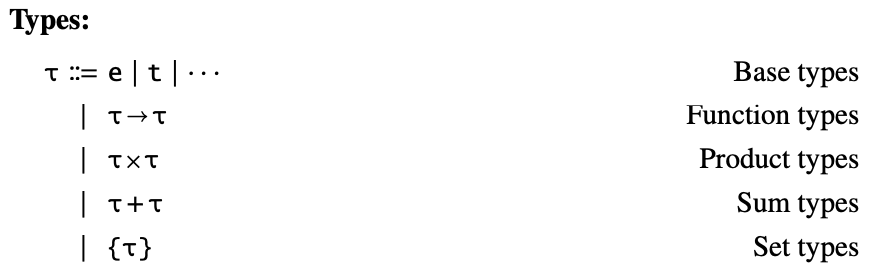
\includegraphics[width=10cm]{clips/1.png}
  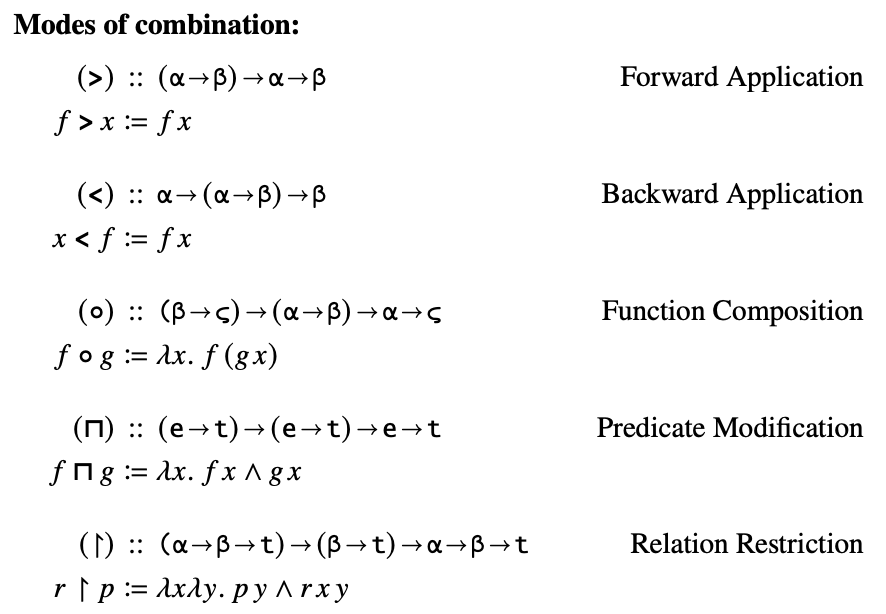
\includegraphics[width=10cm]{clips/2.png}
\end{center}

\begin{itemize}
  \item Without saying more, certain phenomena are difficult to model with this basic framework:
  \begin{exe}
    \ex \label{phenomena}
    \begin{itemize}
      \item context dependence
      \item presupposition
      \item supplemental content
      \item nondeterminism
      \item quantification
      \item focus with association
      \item topicality
      \item dynamism
    \end{itemize}
  \end{exe}
\end{itemize}

\begin{itemize}
  \item These phenomena have something in common. Each contributes additional meaning to consituents that would
  otherwise be type $e$. We might express this additional meaning as follows.
  \begin{center}
    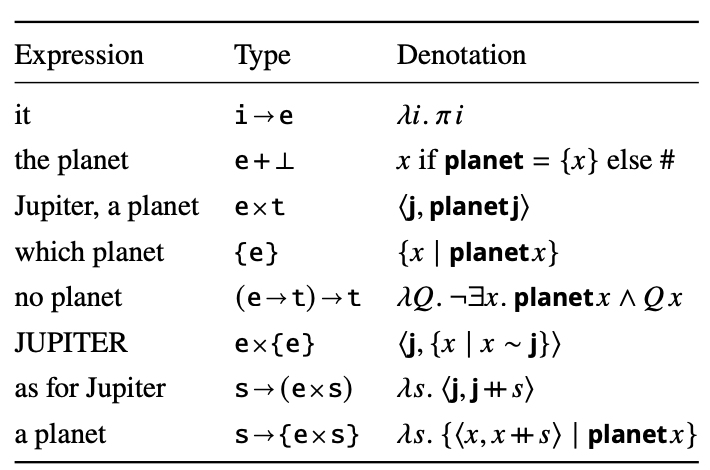
\includegraphics[width=7.5cm]{clips/3.png}
  \end{center}
  \item The basic intuition to develop here is that in each example objects of type $e$ are \textbf{embedded
    in some additional structure}. We will call this additional structure an \textbf{effect}.
\end{itemize}

\section{Functors}

\begin{itemize}
  \item We can say more. Because it's possible to define functions that transform the embedded objects of type $e$
    while preserving the surrounding structure, each of these phenomena is an example of a \textbf{functor}.
  \item We will call such structure-preserving transformations \textbf{maps} and refer to them in symbols as $\bullet$.
    Here are the maps for the environment sensitive and nondeterminate structures, for any type $\alpha$.
  \begin{exe}
    \ex $f \bullet x = \lambda i. f(x \; i)$ \hfill $(e \to \alpha) \to (i \to e) \to (i \to \alpha)$
    \ex $f \bullet x = \{f \; y \mid y \in x \}$ \hfill $(e \to \alpha) \to \{e\} \to \{\alpha\}$
  \end{exe}
  \item We formalize the intuition of structure preservation by requiring maps to satisfy two laws.
  \begin{exe}
    \ex Identity
      \[
          id \bullet x = x
      \]
    \ex Composition
      \[
        f \bullet (g \bullet x) = (f \circ g) \bullet x
      \]
  \end{exe}
  \item In English: mapping the identity function does nothing, while mapping a composite function $f \circ g$ is the same as
    first mapping $g$ and then mapping $f$.
\end{itemize}

\subsection{Putting maps to work}

\begin{itemize}
  \item Why is it worthwhile to observe that these phenomena give rise to functors?
    B\&C observe that their maps can be used to construct composition operations that allow effectful constituents to compose where simple
    function application will not. First some more notational conventions: we will define type constructors for the different effects.
    The type constructors will serve as names for their underlying functors.
\end{itemize}

\begin{center}
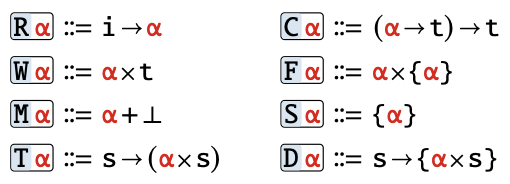
\includegraphics[width=6cm]{clips/7.png}
\end{center}

\begin{itemize}
  \item We will identify each phenomenon in (\ref{phenomena}) with a functor.
\end{itemize}

\begin{center}
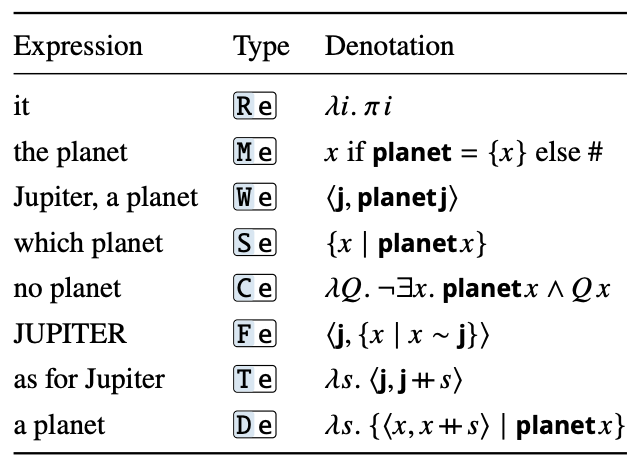
\includegraphics[width=7.5cm]{clips/6.png}
\end{center}

\begin{itemize}
  \item Now we can add forward and backward maps to the grammar, for arbitrary functors $\Sigma$.
\end{itemize}

\begin{center}
  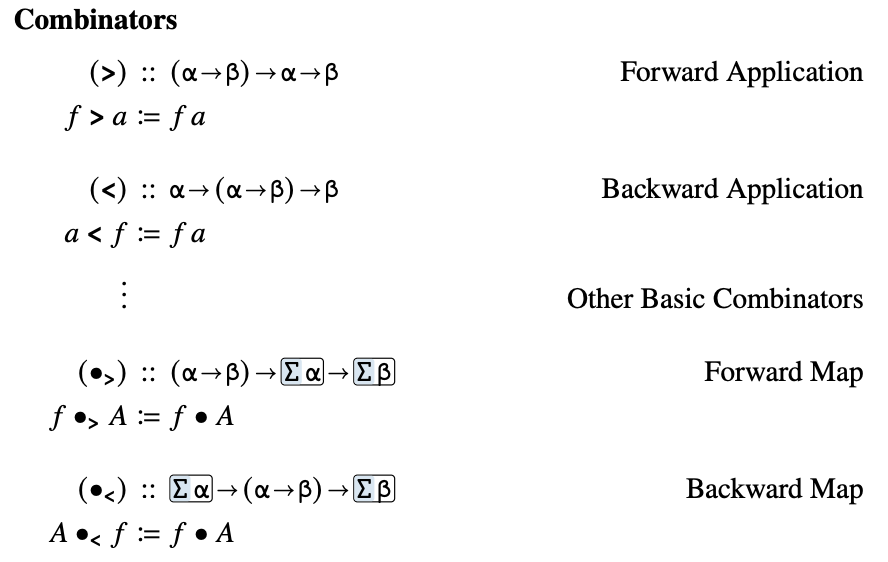
\includegraphics[width=10cm]{clips/4.png}
\end{center}

\begin{itemize}
  \item Here's the immediate payoff: the maps can be used to compose simple functions with effectful arguments.
    We just map the functions over the embedded arguments.
  \begin{exe}
    \ex \hfill \begin{center}
      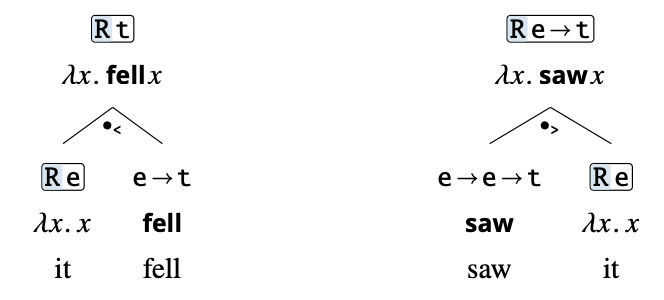
\includegraphics[width=7.5cm]{clips/8.png}
    \end{center}
  \end{exe}
\end{itemize}

\begin{itemize}
  \item We face an immediate problem: there's no way to compose functions that are themselves effectful, as e.g. in (\ref{5}),
    where \textit{saw it} is a context dependent predicate.
    \begin{exe}
      \ex \label{5} Mary saw it.
    \end{exe}
  \item One approach is to introduce Partee's \textsc{lift} operation, and instead of mapping a function
    over an argument, map the argument over the function.
  \begin{exe}
    \ex \textsc{lift} = $\lambda x\lambda k. k \; x$ \hfill $\alpha \to (\alpha \to \tau) \to \tau$
    \ex \hfill \begin{center}
      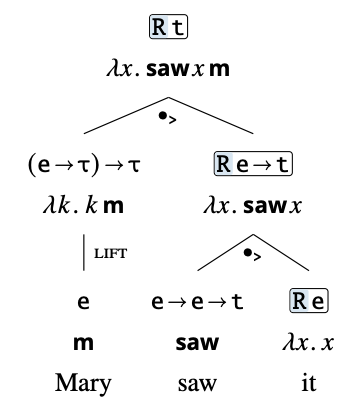
\includegraphics[width=4cm]{clips/9.png}
    \end{center}
  \end{exe}
\end{itemize}

\begin{itemize}
  \item Next problem: it appears that we still can't compose two siblings when both have effects but are otherwise composable.
  \begin{exe}
    \ex \label{9} \hfill
      \begin{center}
        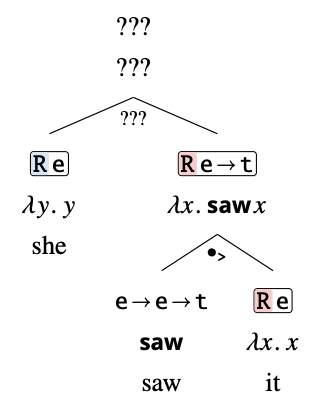
\includegraphics[width=4cm]{clips/10.png}
      \end{center}
  \end{exe}
\end{itemize}

\subsection{Higher Order Effects}

\begin{itemize}
  \item B\&C remark: ``The first step in redressing this unfortunate incomposability is deciding what
  sort of thing (\ref{9}) ought to denote.'' One option is to interpret each pronoun as a separate
  request for an antecedent. Then the meaning of \textit{she saw it} might be of type $i \to i \to t$,
  or $RRt$. B\&C call such a nesting of effects \textbf{higher order}.
  \begin{exe}
    \ex $\intpt{\text{she saw it}} = \lambda x \lambda y. \textbf{saw} \; x \; y$ \hfill $RRt$
  \end{exe}
  \item With some cleverness, it's possible to derive this interpretation with the ingredients we have. We ``map the map''.
  \begin{exe}
    \ex \label{10} \hfill
      \begin{center}
        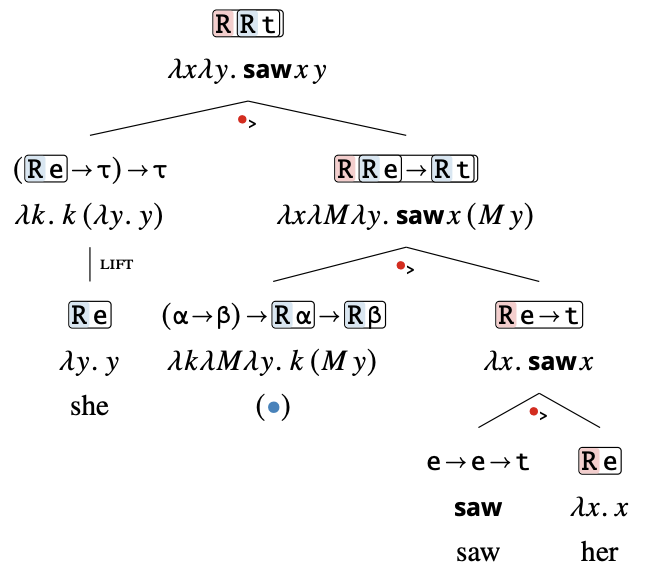
\includegraphics[width=7.5cm]{clips/11.png}
      \end{center}
  \end{exe}
  \item ``Because all of the effects we've introduced are functorial, and the only
  interesting aspects of the derivation are the maps, the tree is a template
  for composition with any of the enriched meanings. For instance, switching R for S
  immediately derives a multiple-wh question''
  \begin{exe}
    \ex \label{12} \hfill
      \begin{center}
        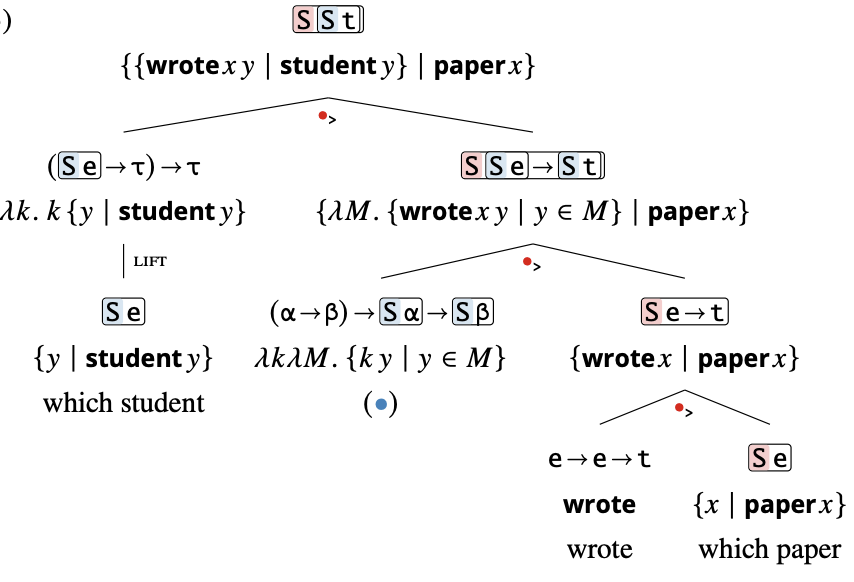
\includegraphics[width=9cm]{clips/12.png}
      \end{center}
  \end{exe}
  \item This even works when function and argument have different effects.
  \begin{exe}
    \ex \label{13} \hfill
      \begin{center}
        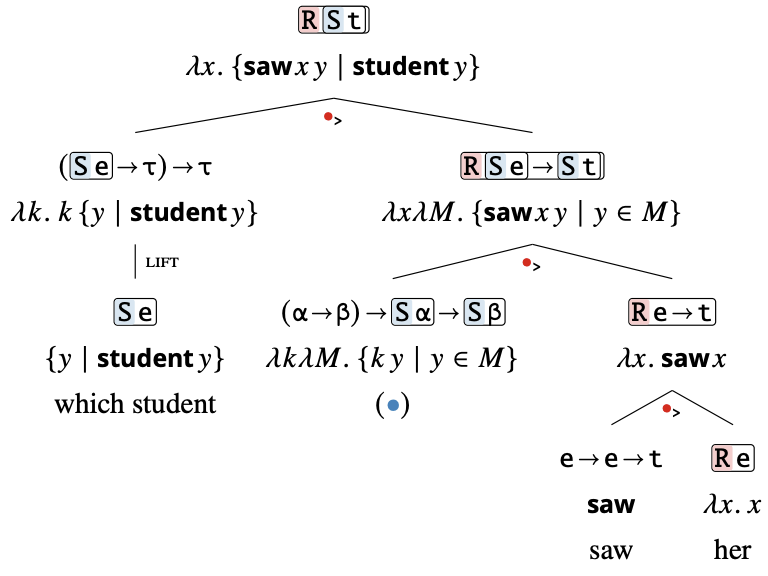
\includegraphics[width=9cm]{clips/13.png}
      \end{center}
  \end{exe}
  \item Now, what about modes of composition beyond function application, e.g. predicate modification?
  \begin{exe}
    \ex \label{14} \hfill
      \begin{center}
        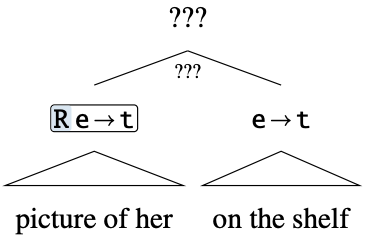
\includegraphics[width=5cm]{clips/14.png}
      \end{center}
  \end{exe}
  \item We might pursue a similar strategy and introduce a PM morpheme.
  \begin{exe}
    \ex \label{15} \hfill
      \begin{center}
        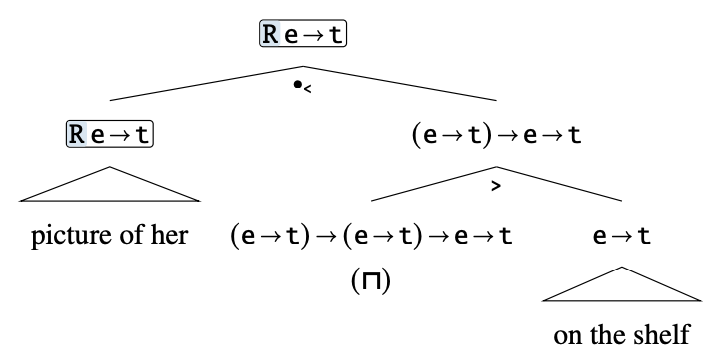
\includegraphics[width=9cm]{clips/15.png}
      \end{center}
  \end{exe}
  \item But there are reasons not to go down this path: ``In this manner, eventually all modes of combination will need to be realized
  lexically. Whether this is syntactically justifiable is open to debate, but it
  certainly increases the distance between the forms that are uttered and the forms
  that are interpreted. And as a practical matter, the resulting combinatorial
  system is admittedly unwieldy.''

  \item Instead, B\&C propose a more systematic approach. We introduce a transformation on composition operations,
    so that ``in general, if there is a mode $*$ that can combine constituents $M :: \sigma$ and $N :: \tau$, then
    there is also a mode to combine constituents $M :: \sigma$ and $N :: \Sigma\tau$, provided $\Sigma$ is a functor.''
    \begin{center}
      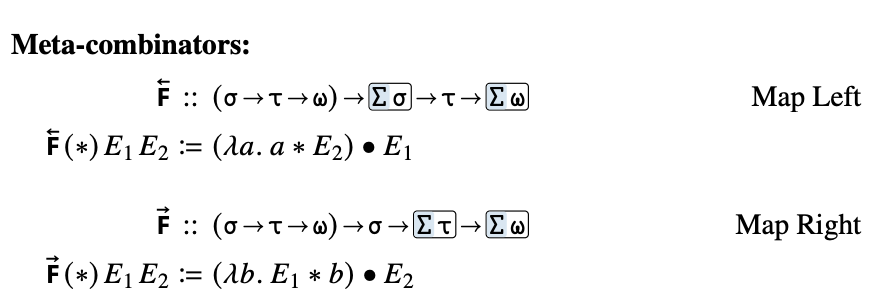
\includegraphics[width=10cm]{clips/16.png}
    \end{center}
  \item We no longer need the bidirectional maps in the grammar, as they can be derived from function application with these meta combinators.
  \begin{exe}
    \ex \label{17} \hfill
      \begin{center}
        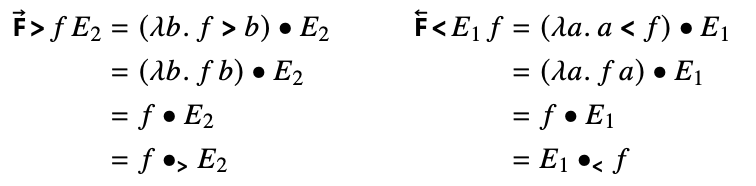
\includegraphics[width=9cm]{clips/17.png}
      \end{center}
  \end{exe}
  \item With the basic composition operations from H\&K and the meta combinators, we can handle FA, PM, \& etc.
  \begin{exe}
    \ex \label{18} \hfill
      \begin{center}
        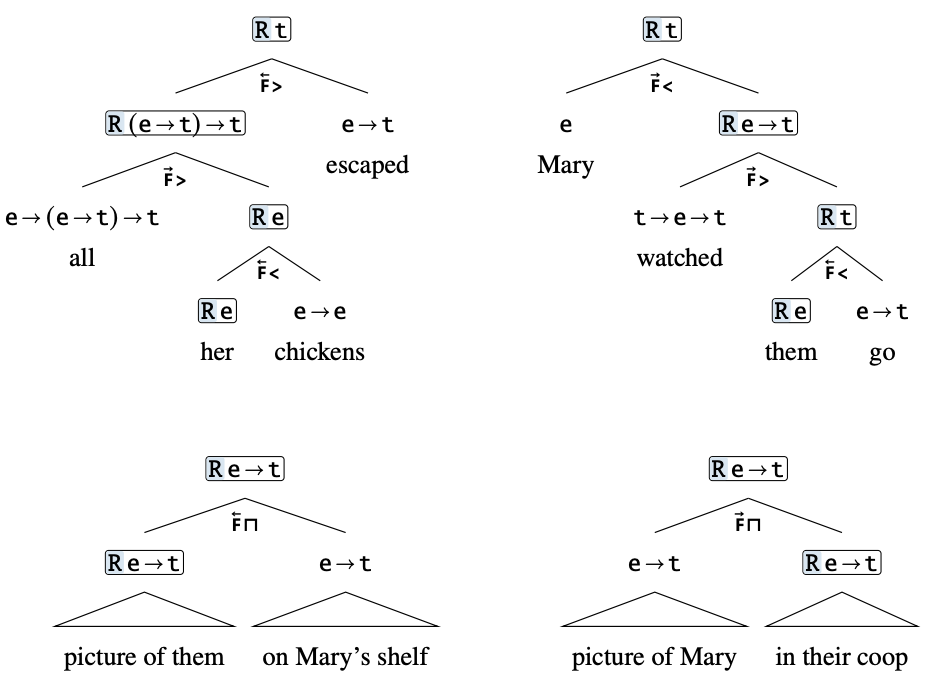
\includegraphics[width=12cm]{clips/18.png}
      \end{center}
  \end{exe}
  \item Interestingly, the $\overrightarrow{F}$ and $\overleftarrow{F}$ combinators can apply to their own output. When the arrows
    go in the same direction, we're able to map over the underlying object(s) of a doubly effectful constituent. In other words,
    we derive a composite map.
    \begin{exe}
      \ex \label{20} \hfill
        \begin{center}
          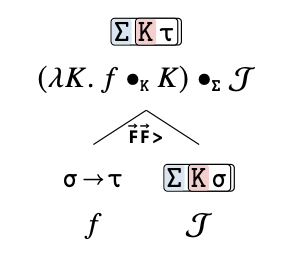
\includegraphics[width=4cm]{clips/20.png}
        \end{center}
    \end{exe}
  \item When the arrows go in opposite directions, we flip the order of effects.
  \begin{exe}
    \ex \label{19} \hfill
      \begin{center}
        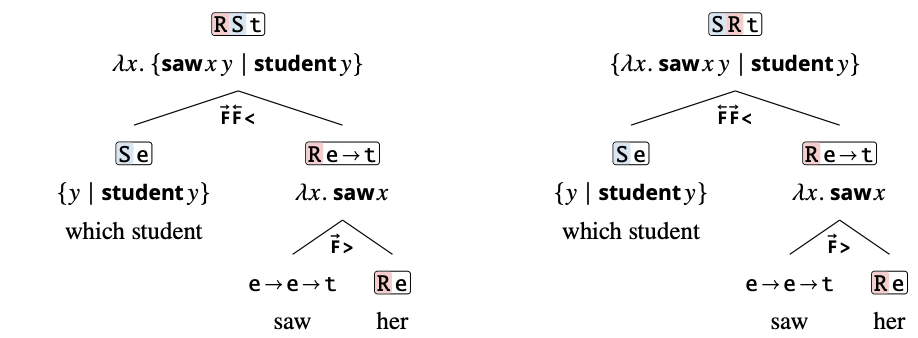
\includegraphics[width=12cm]{clips/19.png}
      \end{center}
  \end{exe}
  \item A final note on the grammar so far: effects always take widest scope, since our composition operations always map ``underneath'' them.
    In (\ref{21}), for instance, the deeply embedded pronoun forces the entire sentence to be context dependent.
  \begin{exe}
    \ex \label{21} \hfill
      \begin{center}
        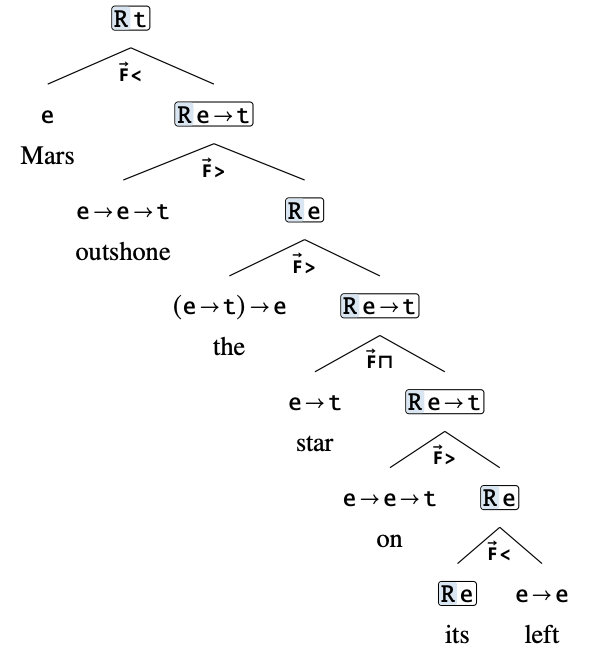
\includegraphics[width=7cm]{clips/21.png}
      \end{center}
  \end{exe}
  \item The same will be true of each effect: no matter how it's embedded, it will force the entire sentence to take its type. In particular,
    effects will not be sensitive to \textbf{island boundaries}. And this is mostly empirically justified, as all of the phenomena we're
    considering -- other than quantifiers -- exhibit exceptional scope.
    \begin{exe}
      \ex Who remembers when who left?
      \ex Mary only gets made when JOHN leaves the lights on.
      \ex Mary hopes that because her cat, named Sassy, is home, John is too.
      \ex Mary's being out of town means that if you don't see John's car, you can be sure nobody's home.
    \end{exe}
\end{itemize}

\pagebreak

\section{Applicative Functors}

\begin{itemize}
  \item Let's reconsider the higher order denotations we settled for above. Ideally, we'd like to derive meanings closer to what
    e.g. \cite{Hamblin1976} and H\&K derive, where the presence of multiple effects, as long as they're the same type, do not force
    the entire sentence in which they occur to be higher order. 
  \begin{exe}
    \ex \label{22} \hfill
      \begin{center}
        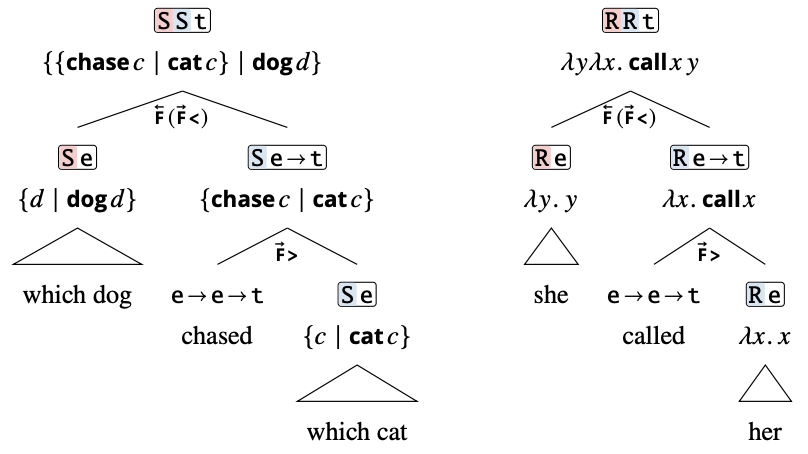
\includegraphics[width=10cm]{clips/22.png}
      \end{center}
  \end{exe}
\end{itemize}

\subsection{Merging effects}
\begin{itemize}
  \item It's straightforward to equip our grammar with generalized-to-the-worst-case pointwise and assignment sensitive composition
  operations that \textbf{merge} the effects of siblings at each composite node.
  \begin{exe}
    \ex Pointwise and Assignment Sensitive Combinators
    \begin{center}
      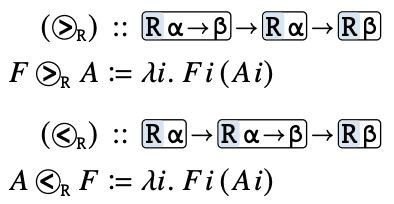
\includegraphics[width=5cm]{clips/24.png}
      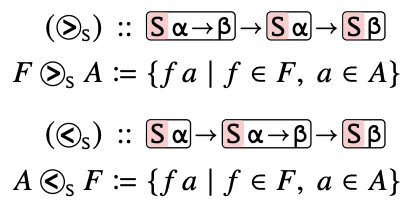
\includegraphics[width=5cm]{clips/25.png}
    \end{center}
    \ex \label{23} \hfill
      \begin{center}
        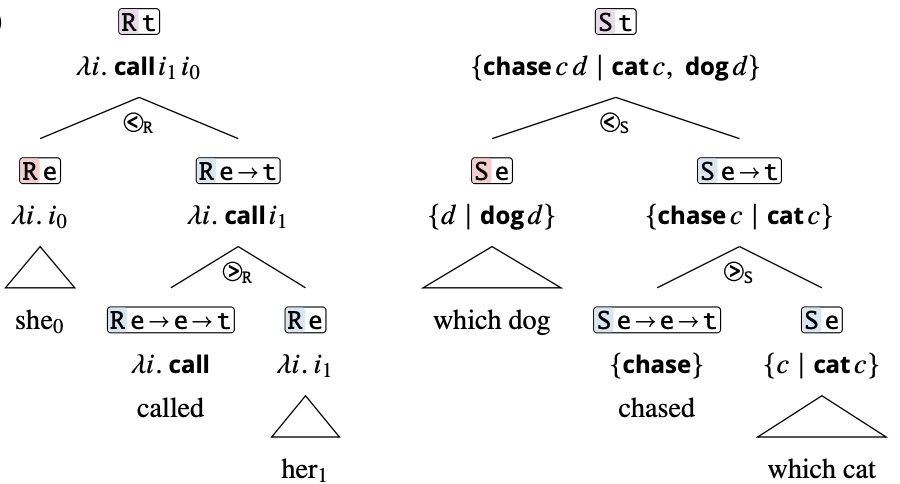
\includegraphics[width=10cm]{clips/23.png}
      \end{center}
  \end{exe}
  \item But B\&C prefer not to generalize to the worst case: ``The rigid, pervasive replacement of ordinary combinatory modes with effect-specific
    variants limits the applicability of the fragment to just the specific effects described. What is gained in uniformity and simplicity is
    sacrificed in generality and extensibility.''
  \item For example: ``Simply mixing the two kinds of phenomena is beyond the reach of either grammar.''
  \item Fortunately, it turns out that the Hamblin and H\&K composition operations are special cases of the operations of a more general structure called an
    \textbf{applicative functor}. A functor is applicative if there exist $\eta$ and $\oast$ functions (pronounced ``unit'' and ``apply'')
    that satisfy the following laws:
    \begin{exe}
      \ex \label{26} Applicative functor laws \hfill
        \begin{center}
          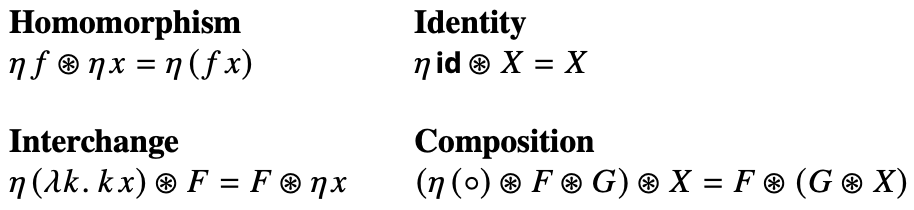
\includegraphics[width=10cm]{clips/26.png}
        \end{center}
    \end{exe}
  \item The $\eta$ and $\oast$ functions for the $R$ and $S$ functors are just the ``lift'' operations -- for incorporating trivially effectful
    constituents -- and the unidirectional versions of the combinators above. We are invited to confirm that they respect the laws in (\ref{26}).
    \begin{exe}
      \ex \hfill
        \begin{center}
          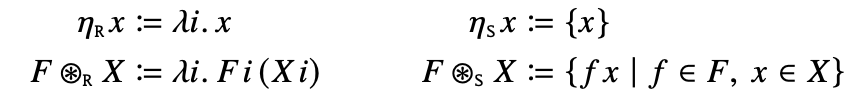
\includegraphics[width=10cm]{clips/27.png}
        \end{center}
    \end{exe}
  \item Each functor that we paired with the phenomena above also gives rise to an applicative. So we could add $\eta$ and $\ostar$ operations to the grammar
   for an arbitrary applicative functor $\Sigma$ and approximate the Hamblin and H\&K grammars.
  \item But we face a problem that parallels our difficulties with regular functors: siblings with nested effects.
    \begin{exe}
      \ex \hfill
        \begin{center}
          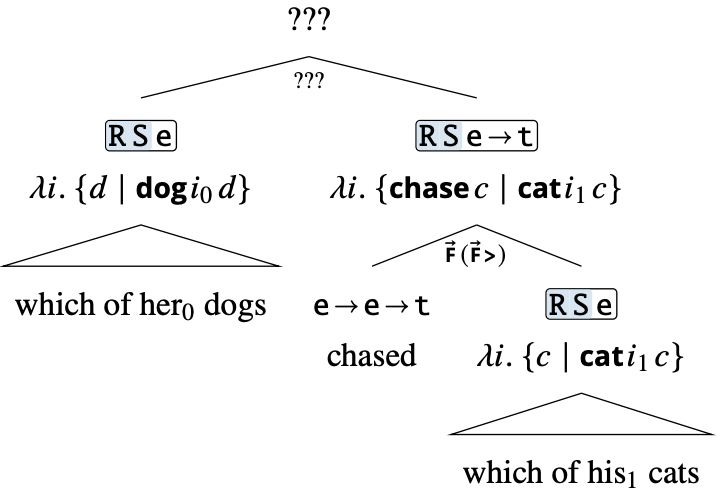
\includegraphics[width=8cm]{clips/28.png}
        \end{center}
    \end{exe}
  
  \item Just as in the previous chapter, the strategy will be to map the new mode of combination below outer effects.
  \item And again, one way of accomplishing this is to let $\oast$ act as a covert operator.
    \begin{exe}
      \ex \hfill
        \begin{center}
          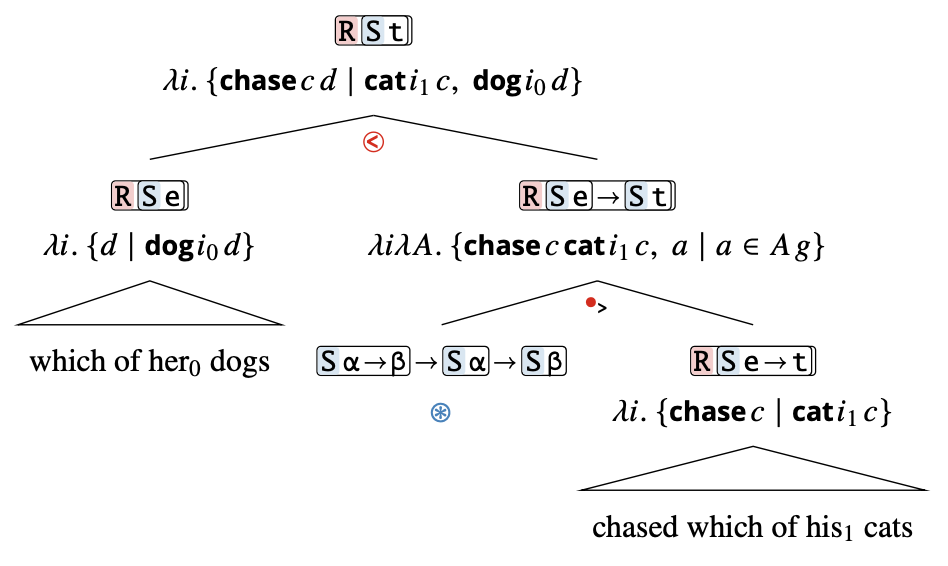
\includegraphics[width=10cm]{clips/29.png}
        \end{center}
    \end{exe}
  \item And another is to introduce a higher order mode of combination. Whenever there is a mode (∗) that might combine
  constituents $M :: \sigma$ and $N :: \tau$, then there should also be a mode to combine constituents $M' :: \Sigma\sigma$
  and $N' :: \Sigma\tau$, so long as $\Sigma$ is an applicative functor.
    \begin{exe}
      \ex Higher order applicative composition \hfill
        \begin{center}
          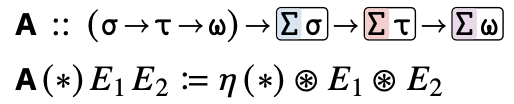
\includegraphics[width=5cm]{clips/30.png}
        \end{center}
    \end{exe}
  \item The generalized pointwise and assignment sensitive modes of composition can be constructed with $\bf A$.
    \begin{exe}
      \ex Higher order applicative composition \hfill
        \begin{center}
          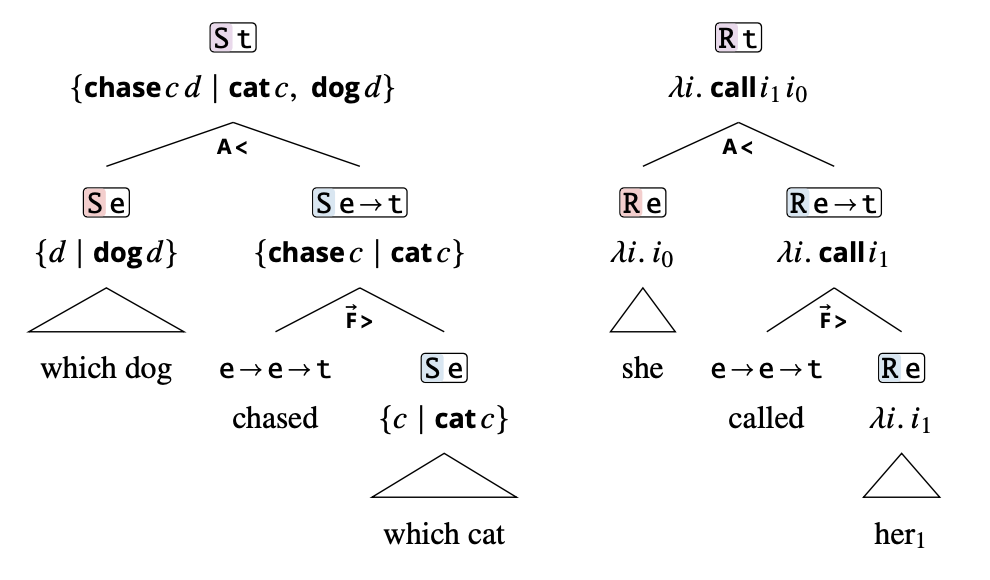
\includegraphics[width=10cm]{clips/31.png}
        \end{center}
    \end{exe}
\end{itemize}

\pagebreak

\begin{itemize}
  \item To compose nested applicative functors, we let $\bf A$ apply twice.
    \begin{exe}
      \ex \hfill
        \begin{center}
          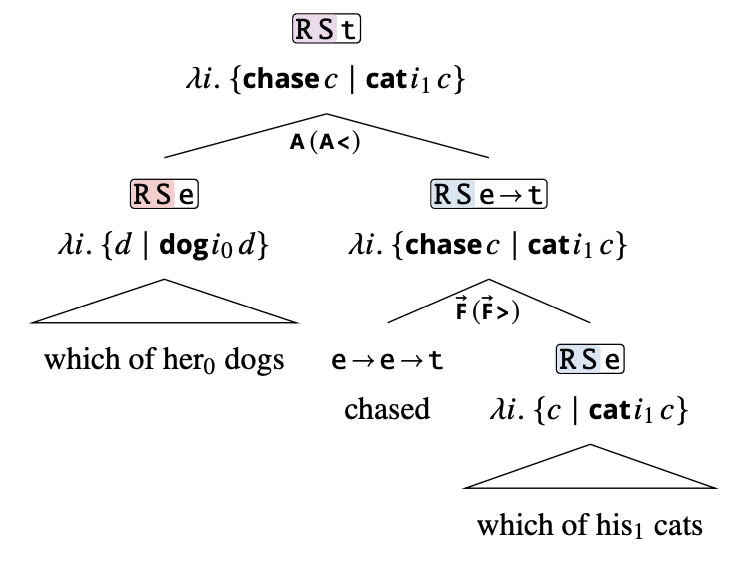
\includegraphics[width=8cm]{clips/32.png}
        \end{center}
    \end{exe}
  \item Having $\overrightarrow{F}$, $\overleftarrow{F}$, and $\bf A$ in the grammar provides
    flexibility. Outer effects may be merged with $\bf A$ while inner ones are mapped over, or vice versa.
    \begin{exe}
      \ex \hfill
        \begin{center}
          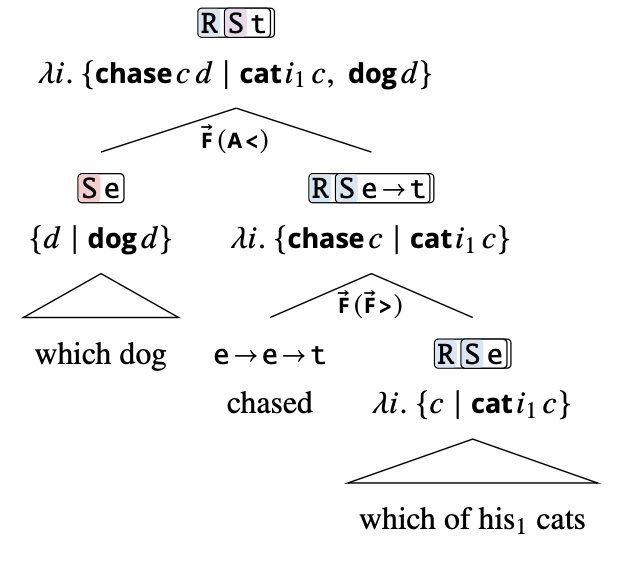
\includegraphics[width=7cm]{clips/33.png}
        \end{center}
      \ex \hfill
        \begin{center}
          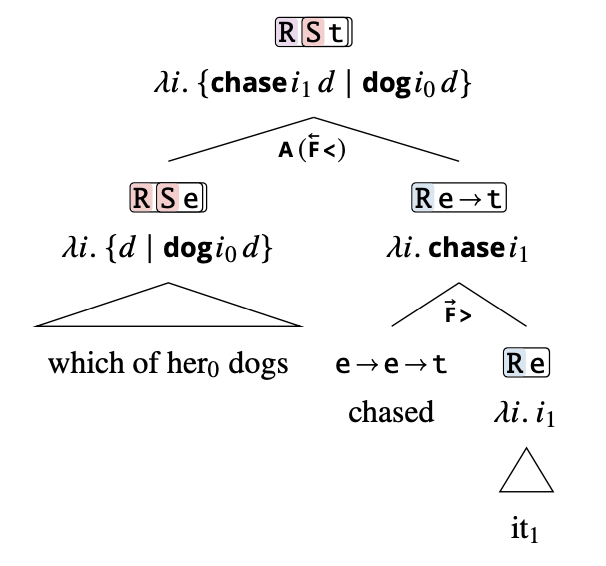
\includegraphics[width=7cm]{clips/34.png}
        \end{center}
    \end{exe}
  
\end{itemize}

\subsection{Selectivity \& eliminating effects}

\begin{itemize}
  \item So far, the grammar offers no way to keep effects from bubbling to the top of a derivation. But there's
  empirical evidence for closure operators, either lexical or covert. In this framework, these items are functions
  that \textbf{eliminate effects}.
  \begin{exe}
    \ex Lexical closure operators \hfill
      \begin{center}
        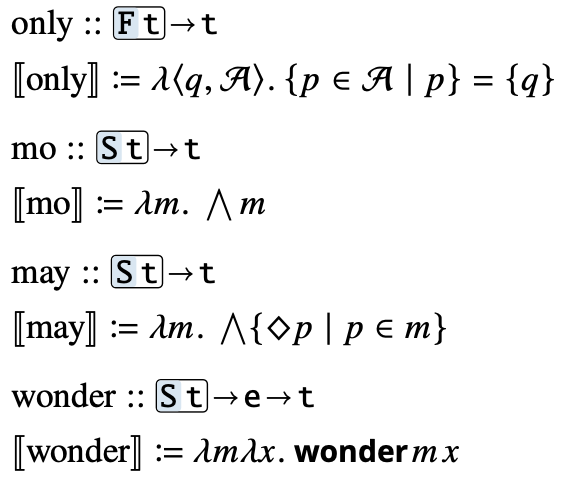
\includegraphics[width=5cm]{clips/35.png}
        \hfill
        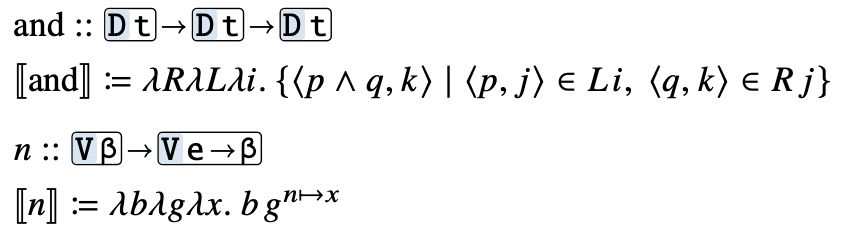
\includegraphics[width=7cm]{clips/36.png}
      \end{center}
      \ex Covert closure operators \hfill
      \begin{center}
        \hspace{-195px}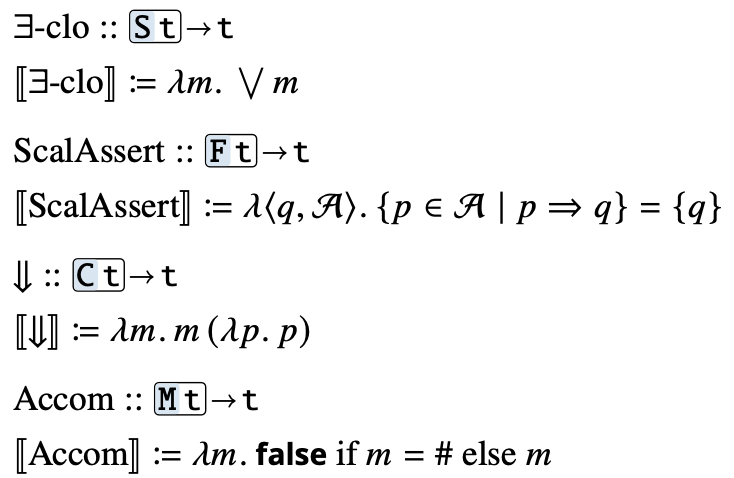
\includegraphics[width=6.75cm]{clips/37.png}
      \end{center}
  \end{exe}

  \item Because applicative composition collapses effects, a closure operator that acts on the result of
    applicative composition will close over every effect in its scope, \textbf{unselectively}.
    \begin{exe}
      \ex \hfill \begin{center}
        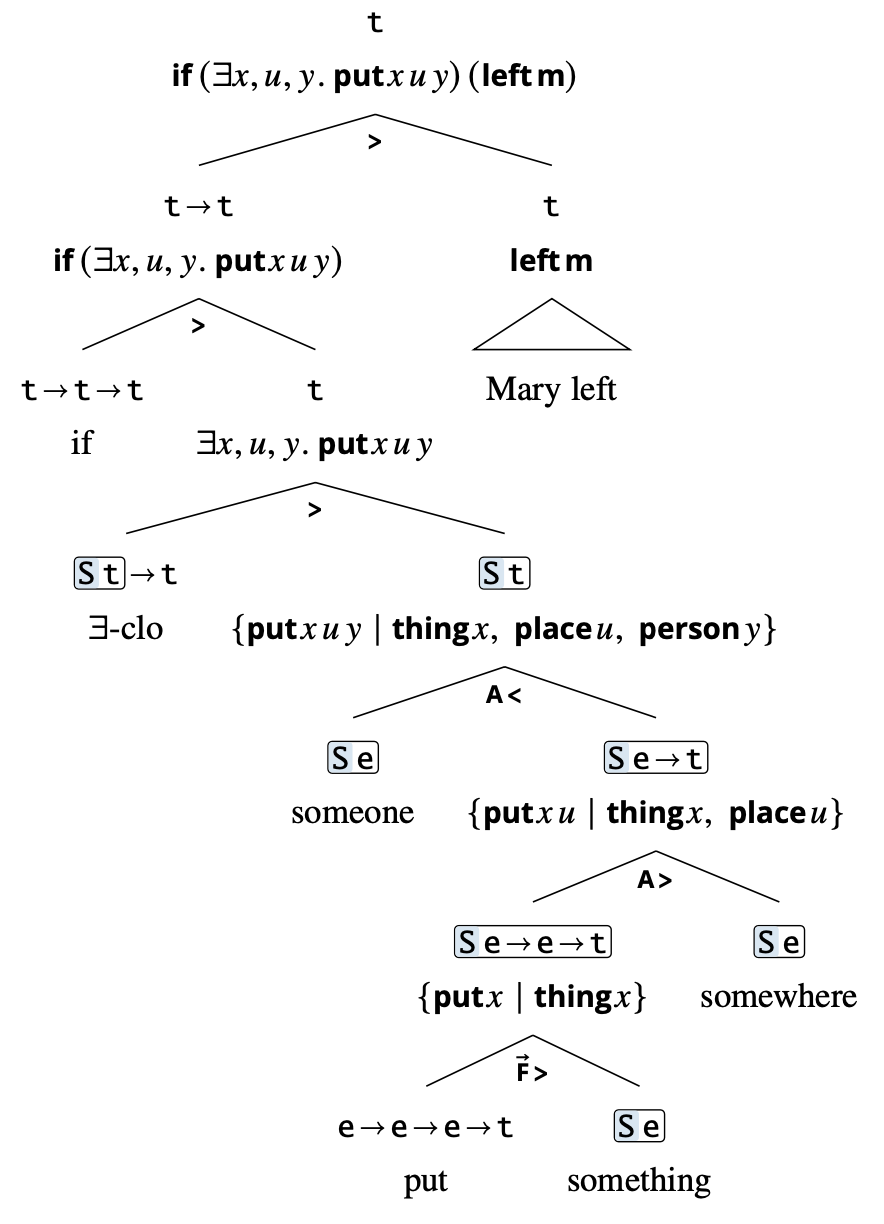
\includegraphics[width=6.75cm]{clips/38.png}
      \end{center}
    \end{exe}
  \item But it's still possible to eliminate effects selectively, and to e.g. allow a single effect to 
    bubble to the top of a derivation, by using an applicative functor's $\bullet$ operation rather than its
    $\oast$ operation.
  \item The derivation below mimics the derivation above except that the alternatives generated by the direct object are consistently mapped-over at every node.
    The alternatives generated by the other two indefinites are merged as above and jointly closed over in the antecedent.
    \begin{exe}
      \ex \hfill \begin{center}
        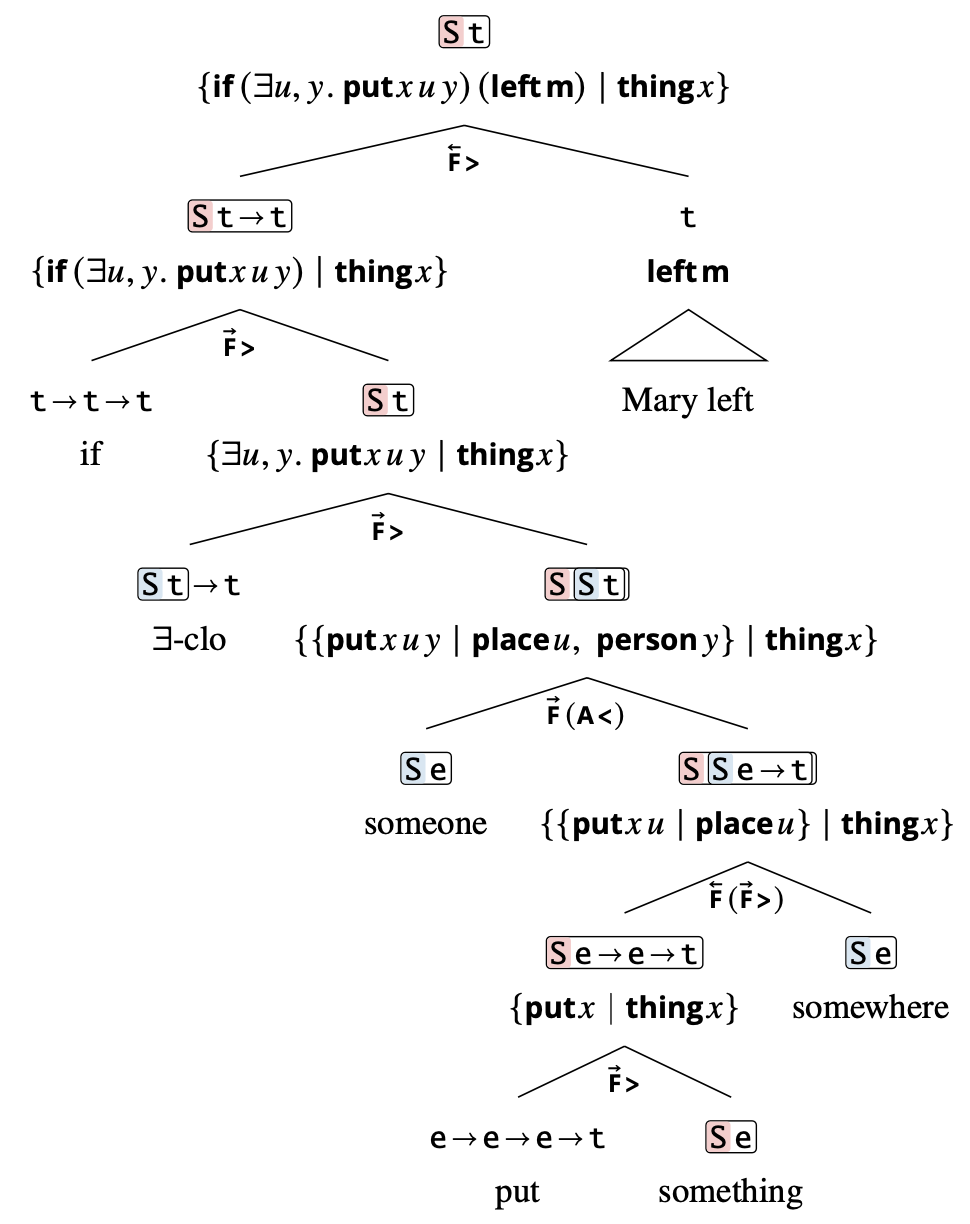
\includegraphics[width=8cm]{clips/39.png}
      \end{center}
    \end{exe}
  \item Now here is a problem: with $\eta$ freely applying in the grammar, we predict that effects can always escape closure operators.
    This will happen if $\eta$ applies to an operator's complement, causing the operator to only eliminate the trivial effect that $\eta$ introduces.
    \begin{exe}
      \ex \hfill \begin{center}
        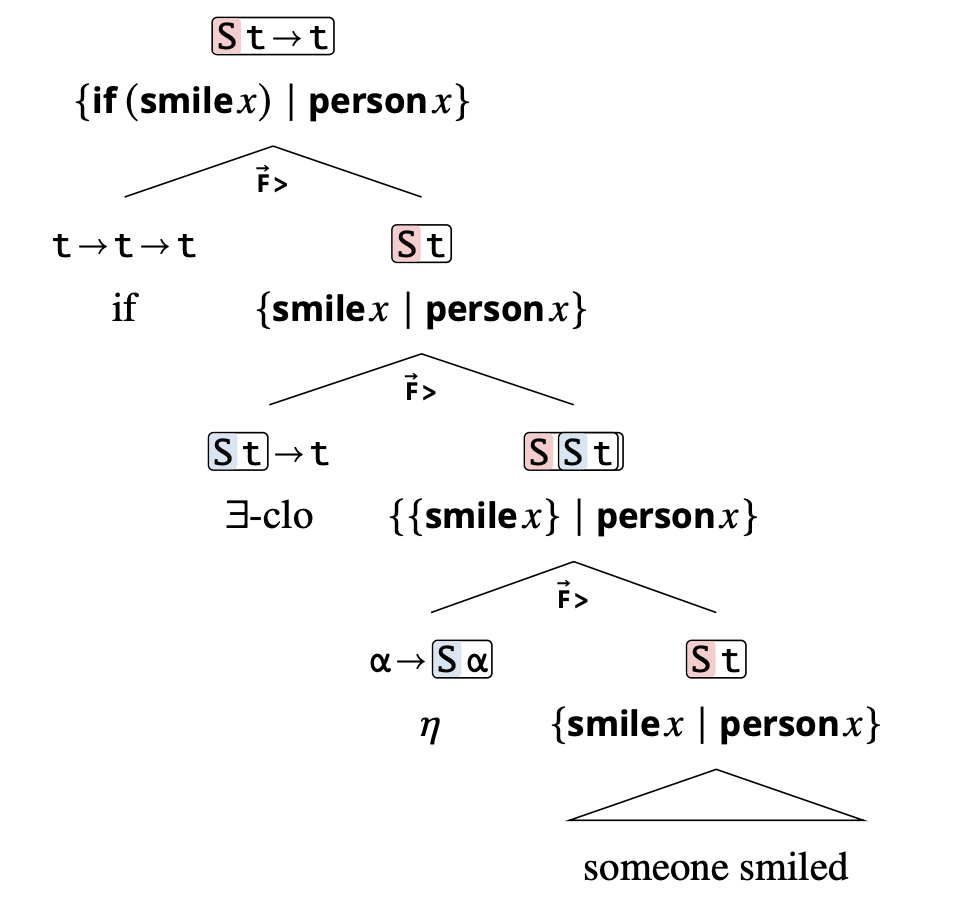
\includegraphics[width=8cm]{clips/40.png}
      \end{center}
    \end{exe}
  \item The solution that B\&C propose is to not let $\eta$ freely apply, but rather to use it only in the course of applying a closure
    operator to a complement that lacks effects: ``the only semantic use for $\eta$ is to feed a closure operator of some sort or another''.
    \begin{exe}
      \ex Closure composition \hfill \begin{center}
        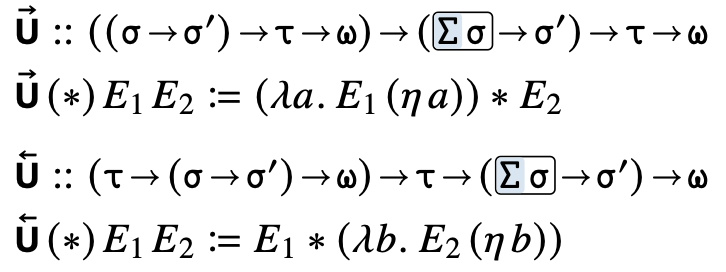
\includegraphics[width=7cm]{clips/41.png}
      \end{center}
    \end{exe}
  \item We use \textbf{U} like so:
    \begin{exe}
      \ex \hfill \begin{center}
        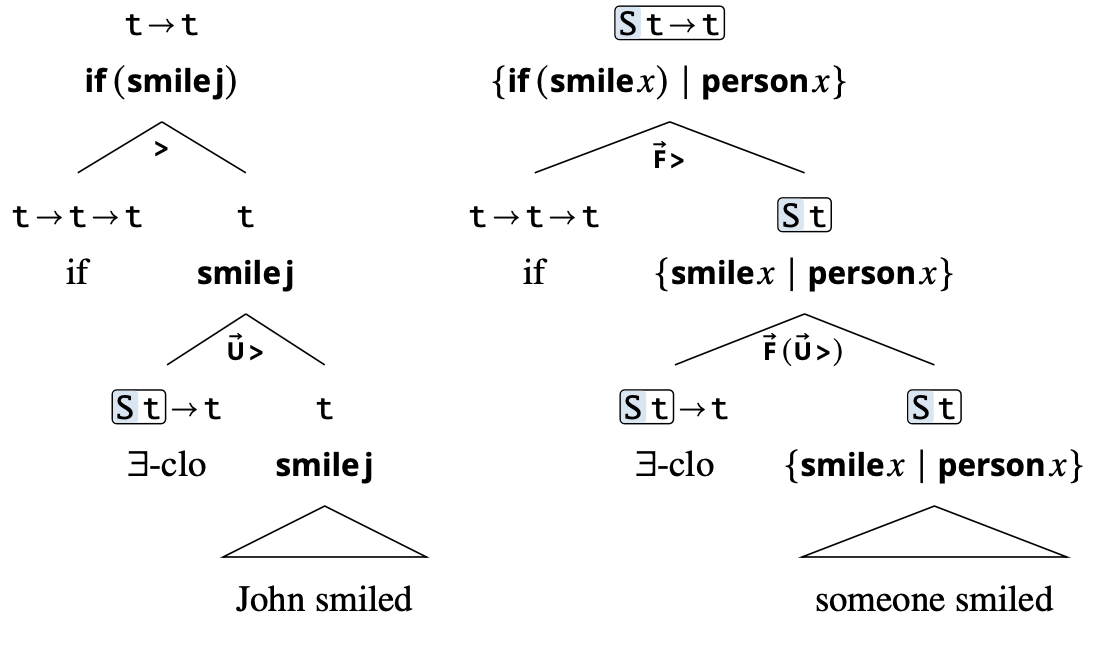
\includegraphics[width=10cm]{clips/42.png}
      \end{center}
    \end{exe}
  \item Here is the grammar so far. ``It's in some sense maximally expressive relative to the applicative structure of an effect. It permits every possible agglomeration or stratification of structure, which in turn means that closure operators may capture anywhere from none to all of the effects in their prejacents.''
    \begin{center}
      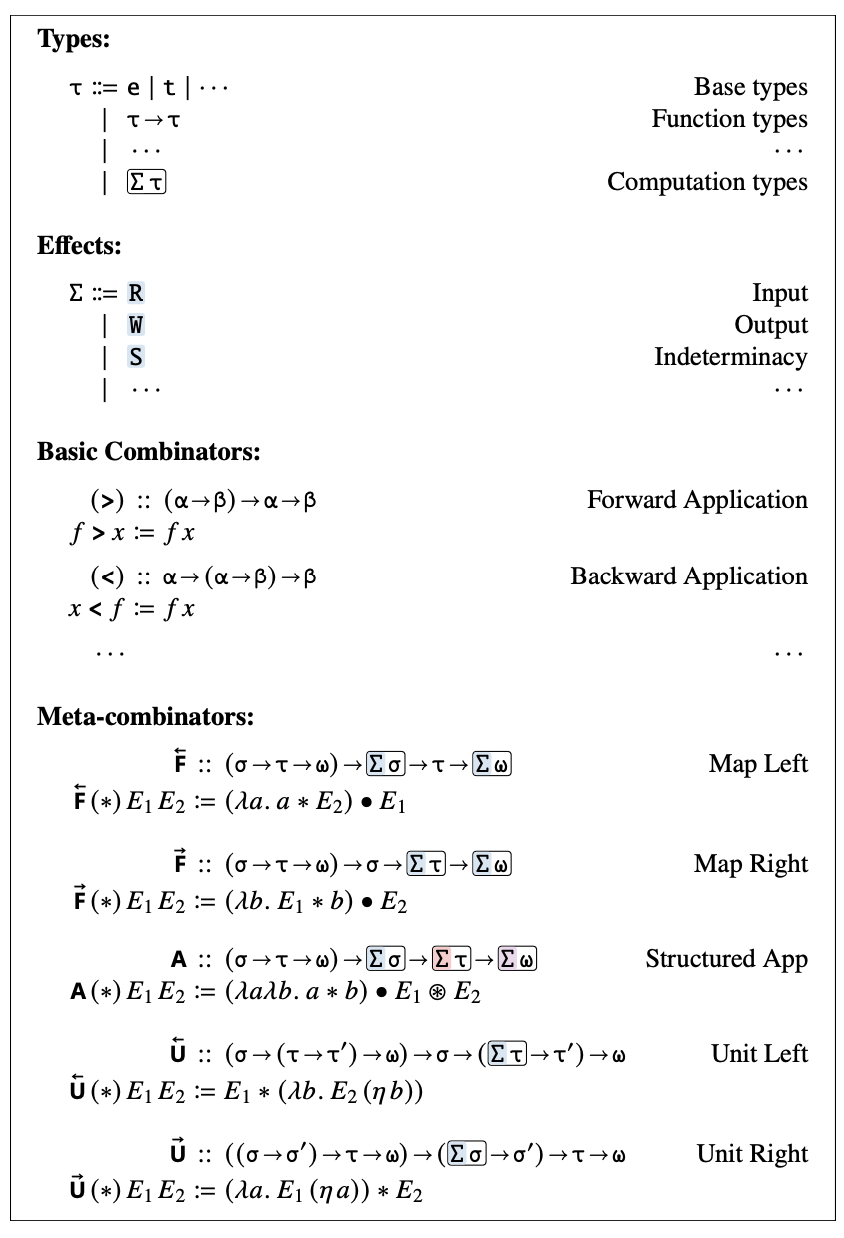
\includegraphics[width=10cm]{clips/43.png}
    \end{center}

  \item We can consider how the grammar behaves when deprived of particular operators.
    \begin{itemize}
      \item With only $\bullet$ , closure operators will need to capture the effect of one and only one constituent.
      \item With only $\oast$, every constituent must be effectful, except closure operators, and closure operators will capture every effect in their scope.
    \end{itemize}
\end{itemize}

\subsection{Commutativity}

\begin{itemize}
  \item The $R$ and $S$ functors are commutative, in the following sense. For any $F :: \Sigma e \to t$ and $X :: \Sigma e$,
    \[ {\bf A} > F X = {\bf A} > X F \]
  \item The $T$ and $C$ functors are not commutative. 
    \begin{exe}
      \ex State updating functor \hfill \begin{center}
        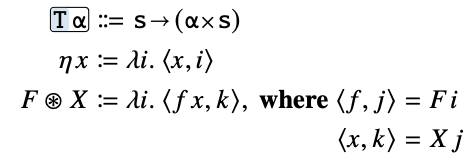
\includegraphics[width=7cm]{clips/44.png}
      \end{center}
      \ex Anaphora with the $T$ functor \hfill \begin{center}
        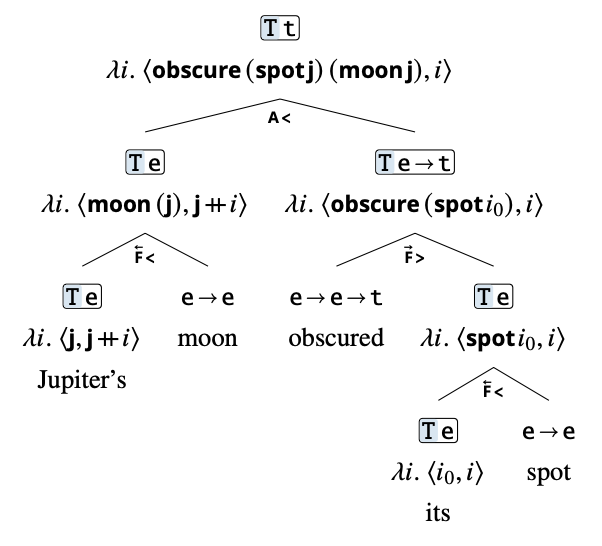
\includegraphics[width=7cm]{clips/46.png}
      \end{center}
      \ex Continuation functor \hfill \begin{center}
        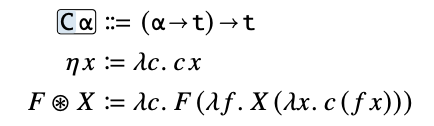
\includegraphics[width=7cm]{clips/45.png}
      \end{center}
      \ex Quantification with the $C$ functor \hfill \begin{center}
        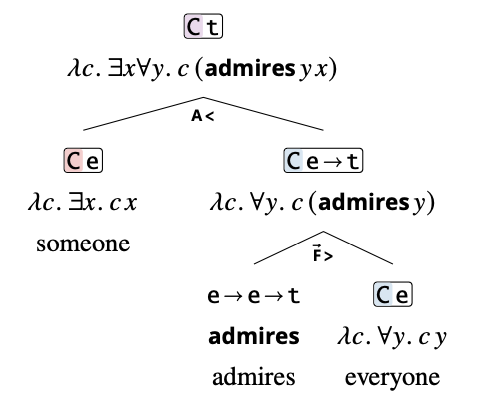
\includegraphics[width=7cm]{clips/47.png}
      \end{center}
    \end{exe}
\end{itemize}

\pagebreak

\bibliography{../refs}

\end{document}